\documentclass[11pt]{article}
\usepackage[tmargin=1in,lmargin=1in,rmargin=1in,bmargin=1.2in]{geometry}
\usepackage{float}

\setlength{\parindent}{0pt}
\setlength{\parskip}{0.25em}
\usepackage{setspace}
\setstretch{1.1}

\usepackage{graphicx} % Required for inserting images

\title{CS520 Project 3: Machine Learning - What Is It Good For?}
\author{Aditya Girish, Rishik Sarkar}
\date{November 10 2023}

\begin{document}

\maketitle

\section{Model 1}

This section is dedicated to our training and testing of Model 1, which is used to predict the best next move for the bot based on the current grid configuration. The subsections shall include the following essential information: the general pipeline of Model 1, a thorough analysis of the training process, and a presentation of the testing process along with any relevant results.

\subsection{Model 1 Pipeline}

I have outlined the general pipeline of Model 1 below, along with any crucial steps taken:

\begin{enumerate}
    \item Import relevant packages and run the \emph{Bot1.ipynb} notebook to gain access to all the setup functions used for Bot 1 in Project 2. None of the functions have been modified, and they allow us to set up the 30x30 grid, randomly place one bot, alien, and crew member, initialize alien and crew probability matrices, move the bot and aliens, update probability matrices, and deterministically determine the best move for the bot. Note that we fixed the ship's layout in terms of the default blocked and open cells, and only the locations of the bot, alien, and crew member change in any given simulation
    \item Simulate Bot 1 similarly to how it was done in Project 2, but collect relevant feature and output vectors to save in a Pandas dataframe (and eventually store as \emph{model\_data\_raw.csv} to be used in training Model 1. I shall go into more detail about the exact feature and output vectors in the next section.
    \begin{enumerate}
        \item To collect enough data, we ran 6000 bots (i.e., until the bot saved the crew or got captured): 30 iterations per simulation and 200 simulations
        \item Through these simulations, we collected a total of 4,132,796 data points
        \item The following hyperparameters were used: alpha = 0.004, k = 3
        \item These were the metric results from the simulation:
        \begin{itemize}
            \item Average Rescue Moves: 585.05
            \item Probability of Crew Rescue: 0.71
            \item Average Crew Saved: 21.3
        \end{itemize}
        \item Note that these values only reflect the final simulation for our data collection phase. Since we modified the input and output vectors several times after the training/testing phase, our simulation hyperparameters, data size, and metrics constantly changed
    \end{enumerate}
    \item Preprocess the collected data and perform train/test splits for the input matrix X and output vector y. We also generated a validity mask for the output vector at this pipeline step, but more later. The following general preprocessing steps were taken:
    \begin{enumerate}
        \item Read the data from \emph{model\_data\_raw.csv} and ensure that the shape is consistent and the data is loading correctly
        \item Remove duplicates from the data to streamline the dataset and remove redundancy. Without this step, the model might memorize frequently occurring data points or become skewed/biased. After this step, the total data points are reduced to 1,787,373
        \item At this point, perform any necessary adjustments to the feature vectors (i.e., dropping/adding columns, normalizing data, etc.). Since we were confident about our features during our final collection process, we did not make any modifications to the collected data
        \item Separate the data into the input matrix X and the output vector y (with the output being the last column and the input being all the other columns). Note that PCA or other feature engineering methods could also be performed in this step
        \item Divide the X and y dataframes into train and test sets with an 80/20 split, respectively. At this point, we also checked that all five classes were equally represented in each set
        \item Finally, generate the validity mask vector dataframes for the train and test sets. Each row in the validity mask corresponds to the same row in the X\_train and X\_test datasets, and essentially represents the neighbors that the bot can move to given the board's open and closed cells. The following process was used to generate this validity mask:
        \begin{enumerate}
            \item For any given datapoint, use the bot\_x and bot\_y features (that represent the bot's current coordinates) along with an empty grid state to determine what neighbor cells count as valid moves for the bot
            \item Each datapoint in the valid dataframes is represented as a list in the form of [$c_1, c_2, c_3, c_4, c_5$] depicting the up, down, left, right, and bot cells, respectively. Each $c_i$ is 0 if the corresponding relative neighbor is an invalid move and 1 if the bot can move to it. The significance of this vector will become clear in the next section
        \end{enumerate}
    \end{enumerate}
    \item Train the logistic regression model on the X\_train + y\_train dataset and save the updated W and b values for Model 1. Since I will go into the input, output, model spaces as well as the learning techniques in the next section, this point is dedicated to discussing the final training hyperparameters:
    \begin{itemize}
        \item alpha (learning rate) = 0.01
        \begin{itemize}
            \item We additionally tried 0.001 and 0.05, but 0.01 seemed to be optimal. A value of 0.001 caused the model training to be prolonged, whereas 0.05 caused the loss to fluctuate due to overstepping
        \end{itemize}
        \item epochs = 50
        \begin{itemize}
            \item We tried several other epoch values, but 50 seemed an ideal number for the loss to decrease until it became asymptotic
        \end{itemize}
    \end{itemize}
    \item Test Model 1 on the testing dataset with the updated W and b values and calculate the accuracy of predicting the best move. I shall discuss our findings in more detail in the Results section, but we generally saw no indication of overfitting and achieved decent training and testing accuracy
    \begin{itemize}
        \item Additionally, to confirm that the decrease in loss caused an increase in accuracy (i.e., the model was improving), we calculated the training and testing accuracy using randomized weights and biases and averaged the results over 100 calculations. Overall, we were able to find a significant improvement in both training and testing accuracy using the trained weights than the randomized weights, thus indicating that the model truly learned
    \end{itemize}
    \item Simulate Model 1 through a new bot called Mimic-Bot1 that utilizes the logistic regression model's predictions to determine the next move for the bot by utilizing the same features as the trained model. Here is a general outline of the process:
    \begin{enumerate}
        \item Create the Mimic-Bot1 simulation function identical to the Bot1 simulation function, but instead of using the deterministic \emph{determine\_move()} function defined in \emph{Bot1.ipynb}, predict the next move at each timestep by using Model 1 with a dataframe input containing features extracted from the current ship configuration (similar to the data collection function)
        \item Test the Mimic-Bot1 simulation out against the Bot1 simulation function similar to how the testing was performed in Project 2 with Bot 1 and Bot 2, and store the collected average metrics for each bot
        \item We ran 400 bots for both Bot 1 and Mimic-Bot1: 20 iterations per simulation and 20 simulations
        \item The following hyperparameters were used: alpha = 0.004, k = 3
        \item Importantly, we calculated a validity mask for every X input, and used a prediction function that applied the validity mask to the output to ensure that the bot would remain within bounds
        \item Later, we added a stochastic element to the prediction provided by Model 1. In essence, we generated a random number between 1 and 5 and returned a random valid move if the number was 1 (i.e., 20\% of the time). This modification accounted for situations where Mimic-Bot1 got stuck in an endless loop. Consider the following scenario: The bot is in a cell from which the highest probability neighbor is "up," but following the highest probability from "up," the bot is taken back to the original cell. By adding slight randomness, Mimic-Bot1 can escape such loops by taking unexpected actions
    \end{enumerate}
\end{enumerate}

\subsection{Training Process}

In this section, I shall outline the training process for Model 1, including the input and output features, the model space, the loss function, and the training algorithm we used.

\subsubsection{Input Space}

The data that was collected and represented as input features in our final model are as follows:

\begin{enumerate}
    \item The bot's current x and y coordinates as two individual integer features \emph{bot\_x} and \emph{bot\_y}
    \begin{itemize}
        \item Previously, we naively tried storing this feature as a string of a tuple but realized that separating the coordinates into two numerical features was the only way we could use logistic regression since they must be multiplied by weights
        \item We also once tried removing the features altogether, but we achieved better accuracy by including them
    \end{itemize}
    \item The alien probabilities for all neighboring cells (and the current bot cell) as float32 features. They are in the order: \emph{alien\_up}, \emph{alien\_down}, \emph{alien\_left}, \emph{alien\_right}, \emph{alien\_stay} representing the probabilities of the alien being in the up, down, left, right, and bot cells respectively. We tried several other versions for the alien probabilities, as outlined below:
    \begin{itemize}
        \item At first, we included the entire flattened alien probability matrix (which was stored as a dictionary in the simulation), which meant that every individual open cell key within the dictionary was represented by a feature in the form \emph{alien\_[str(key)]} with the probability value stored as a float64 (and later float32). This approach resulted in around 1,219 features (including the others), which caused our data collection phase to take an extremely long time and resulted in an 18 GB CSV dataset!
        \item Understanding that the professor mentioned a similar approach within office hours and that having as much information as possible could not hurt, we attempted the entire training, testing, and simulation process with this expansive dataset, only to find that the accuracy was still very low. I dove into the simulation results and the calculated weights to resolve this issue (and potentially streamline the process). I realized that a significant problem was the low variance between the values of each feature over all datapoints and a predominance of tiny and zero probabilities. To resolve this, I attempted to filter out and keep only features with variance above a certain threshold (0.01, 0.001, 0.0001, etc.) but did not see a significant change over several training and testing periods.
        \item As a last resort, I even attempted to use Principal Component Analysis (PCA) for dimensionality reduction by following these steps:
        \begin{enumerate}
            \item Standardized data and computed the covariance matrix
            \item Performed eigenvalue and eigenvector decomposition and sorted eigenvalues in descending order
            \item Selected the top 10, 100, and 200 eigenvectors (over three different tests)
            \item Transformed the original dataset based on the projection onto the relevant eigenvectors
        \end{enumerate}
        However, I ran into issues with the eigenvector computations due to the low variance in the dataset (all PCs contained 0s for any sub-dataset with over 50,000 datapoints and \emph{k\_components} = 100), and I was not sure how to reflect the projection onto the collected datapoints during the simulation, so we chose to abort the process ultimately
        \item Finally, looking into the process we utilized in deterministically finding the best next move in Project 2, we decided only to consider the up, down, left, right, and current cells, which also significantly improved the data collection efficiency, reduced the CSV file size and allowed for more datapoints, and increased the overall training and testing accuracy. To account for the low probabilities within the remaining five alien probability features, we normalized them so that they summed up to 1 (unless their sum was 0 before)
    \end{itemize}
    \item The crew member probabilities for all neighboring cells (and the current bot cell) as float32 features. They are in the order: \emph{crew\_up}, \emph{crew\_down}, \emph{crew\_left}, \emph{crew\_right} representing the probabilities of the crew member being in the up, down, left, and right cells respectively. All the variations that we tried out for alien probabilities were also applied to the crew probabilities, with a few changes:
    \begin{itemize}
        \item We decided to drop the \emph{crew\_stay} column since the crew probability was guaranteed to be 0 for the bot's current cell. We attempted to remove the corresponding \emph{alien\_stay} column as well, but saw no significant improvement in performance or accuracy
        \item Note that crew member probabilities were typically higher than alien probabilities since the only situations where alien probabilities were high were when the alien was within the detection square sensor, whereas crew probabilities were likely non-zero. Thus, normalizing crew probabilities seemed to have a more significant impact than alien probabilities
    \end{itemize}
    \item Per the professor's announcement, we added features reflecting the distance from the bot's neighboring cells to the two cells with the highest alien and crew member probabilities, respectively. Hence, we included ten additional features: \emph{d\_alien\_up}, \emph{d\_alien\_down}, \emph{d\_alien\_left}, \emph{d\_alien\_right}, \emph{d\_alien\_stay}, \emph{d\_crew\_up}, \emph{d\_crew\_down}, \emph{d\_crew\_left}, \emph{d\_crew\_right}, \emph{d\_crew\_stay} stored as float32 values. To collect these features, we had to modify our simulation function slightly and add two new helper functions:
    \begin{itemize}
        \item We initially found the key cell with the highest probability for the crew and alien matrices and then calculated the distance from each direction cell to the respective max probability cells (if the direction cell was open). Instead of running BFS every time, we utilized the crew sensor function defined in Project 2 (without actually storing the crew detection results) and saved the \emph{d\_list} for the open direction cell within the \emph{d\_lookup\_table} to make the simulation more efficient 
        \item To recap, the \emph{d\_lookup\_table} dictionary stores cell tuples as keys and the distances to all other open cells as their respective values in the form of dictionaries. We did this so that the distance dictionary (i.e., \emph{d\_dict}) did not need to be recalculated using BFS every time. Using the crew sensor and updating the \emph{d\_lookup\_table} improved the efficiency of the distance determination process and the entire simulation
        \item After collecting the distance values for all direction cells from the max alien and crew probability locations, we stored the feature values as $1/$\emph{d\_direction\_cell} if the direction cell was open, and 0 if not
        \item Since we did not use the actual alien and crew member locations within our calculation process or as features, I am confident that we met the criteria of the project
    \end{itemize}
    \item The binary values for whether the bot received a beep or not from the alien sensor and crew sensor as two features: \emph{alien\_detected} and \emph{crew\_detected}
    \begin{itemize}
        \item The values for the features are 0 if the corresponding sensors return False and 1 if they return True
        \item Although these did not make much sense to include at first, removing them caused the accuracy to decrease. This illogical result might have occurred because of the sparsity of the dataset and the model learning from features with more variance, such as these two. We kept the features, however, and have not observed a decrease in accuracy, especially after adding in the new features introduced above
    \end{itemize}
\end{enumerate}

Overall, our final Model 1 was trained on 23 distinct features stored as integers and float32 values, as depicted above.

\subsubsection{Output Space}

The output space for Model 1 consisted of the best move made by the bot with a given ship configuration. The only thing that changed was how it was encoded:

\begin{itemize}
    \item At first we naively tried to store the output value as a string encoding of the tuple cell. In hindsight, this was clearly not the correct technique, since it would have to be predicted from a combination of numerical weights and input vectors
    \item Then, we tried to encode the output values as integers from 1 to 5, with 1 = up, 2 = down, 3 = left, 4 = right, and 5 = stay in place. This process seemed fine at first, but it had two issues. Firstly, the model might find implicit relationships between two such output values. For example, 1 + 2 = 3, but up + down is not left. I don't even know what that means. Similarly, the model might define a sense of ordinality between the output classes, such as 1 $<$ 2 $<$ 3. These relationships could be dangerous to the training process
    \item Ultimately, we decided to one-hot-encode the output value as a list with five binary values. In this case, up = [1,0,0,0,0], down = [0,1,0,0,0], left = [0,0,1,0,0], right = [0,0,0,1,0], stay = [0,0,0,0,1]. This conversion allowed us to introduce a linear relationship between all the classes and removed the possibility of unnecessary dependencies. Also, one-hot-encoding allowed us to make the validity mask generation and application process much simpler during the loss and gradient calculation and prediction phases
    \item Within the CSV itself, the one-hot-encoded output values are stored within double quotes, but the dataset loading process ensures that the output vector is one-dimensional and contains the list of encodings per datapoint
\end{itemize}

\subsubsection{Model Space}

To map from the input to the output, we considered a multiclass logistic regression model with softmax activation. Essentially, here are the steps followed by the logistic regression model:

\begin{enumerate}
    \item During training, the model receives an input vector $X_i$, and uses a linear combination of the vector with weights (W) and bias (b) to compute the output $z = X_i \cdot W + b$
    \item The output is then transformed into probabilities for each class via the softmax function. Essentially, the probability for class with index $i$ given the output value, and the fact that there are 5 classes (up, down, left, right, stay), is computed as such:
    \begin{itemize}
        \item softmax($z_j) = \frac{e^{z_j}}{\sum_{i=1}^{5} e^{z_i}}$
    \end{itemize}
    This ensures that the probability is distributed over the 5 possible moves
    \item Bonus:
    \begin{itemize}
        \item For our bonus, we used the scikit-learn \emph{LogisticRegression} library to create a multiclass model using a \emph{saga} (Stochastic Average Gradient Augmented) solver due to the extensive training dataset. The scikit-learn model also uses the softmax activation function I mentioned earlier and uses L2 regularization to prevent overfitting (which we shall go into more detail about in the next section). We used the same dataset as the logistic regression model we built from scratch. We used 1000 iterations in our training, and all the other processes were identical unless noted otherwise
    \end{itemize}
\end{enumerate}

\subsubsection{Loss}

As a multiclass classification model, Model 1 uses a cross-entropy loss function that measures the difference between the true and predicted probability distributions for the classes in the following way:

\begin{enumerate}
    \item As parameters, we input the predicted \emph{chosen\_action} vector and the true \emph{chosen\_action} vector as well as the validity mask that, as mentioned in Section 1.1, is one-hot-encoded to depict the valid moves for the bot
    \item At first, the validity mask vector is element-wise multiplied by the predicted probability vector $\hat{y}$. This operation is done so that the probabilities for invalid bot moves become 0. Then, the probabilities in $\hat{y}$ are normalized, so the sum remains 1. This process is crucial since it aligns the learning process of Model 1 with the constraints imposed by the simulation
    \item After that, the cross-entropy loss is calculated for each one-hot-encoded datapoint (with five classes) in true output vector $y$ and predicted output vector $\hat{y}$ by using the following equation:
    \begin{itemize}
        \item $L(y, \hat{y}) = - \Sigma_{i=1}^{5} y_i \cdot log(\hat{y_i} + \epsilon)$
        \item In this case, $\epsilon$ refers to a small constant (1e-15) to ensure that log(0) is not being calculated, and $L(y,\hat{y})$ is the loss for that particular datapoint
    \end{itemize}
    \item Finally, the loss for each datapoint is added up and averaged (divided by n, where n is the number of datapoints). Since the calculations take place for the entire vectors at once, this operation is implicit
    \item Bonus:
    \begin{itemize}
        \item We did not define the loss function explicitly since we used the default scikit-learn \emph{LogisticRegression} library. However, as mentioned earlier, we used L2 regularization, which, as I understand it, added a penalty to the loss function equal to the sum of the squared values of the calculated weights with a specific regularization strength. Additionally, we used L2 over L1 regularization because we found through research that L1 is better for feature selection, but since we already have very few features (after reducing the original 1,219 features to 23), L2 seemed to be a better fit for the use case
        \item Note that because we could not figure out how to account for one-hot-encoded output vectors within scikit-learn, we were forced to use integer representations for each output class (based on the index in the one-hot-encoding). For example, up = 0, down = 1, and so on. We were also unable to apply the validity mask during loss calculations, instead opting to use it only during the simulation
    \end{itemize}
\end{enumerate}

\subsubsection{Training Algorithm}

The training algorithm for Model 1 uses gradient descent to minimize the cross-entropy loss function. The algorithm iteratively updates the weights and biases to yield the lowest possible loss value. Here are the steps we followed to implement it:

\begin{enumerate}
    \item As parameters, we input the predicted output vector $\hat{y}$, the true output vector $y$, the input matrix $X$, as well as the validity mask mentioned earlier
    \item Similar to the loss function, we first multiply the validity mask vector by the predicted probability vector $\hat{y}$ to reduce invalid moves to 0 and then subsequently normalize the valid probabilities so that the sum is 1
    \item Then we calculate the gradient of the loss function with respect to the weights $W$ and bias $b$ as follows:
    \begin{itemize}
        \item $\nabla_{W} L = \frac{1}{n} X^{T} \cdot (\hat{y} - y)$
        \item $\nabla_{b} L = \frac{1}{n} \Sigma_{i=1}^{n} (\hat{y_i} - y_i)$
    \end{itemize}
    In this case, $X$ is the input matrix of size $n \times m$, and $\hat{y}$ and $y$ are the predicted and true output vectors of size $n \times 5$ (since there are five classes in the one-hot-encoding). Additionally, $L$ is the loss function that was calculated earlier
    \item Finally, after we have calculated the gradient of the loss function with respect to both $W$ and $b$, we can use them to update the weights and bias in the following way:
    \begin{itemize}
        \item $W = W - \alpha \cdot \nabla_{W} L$
        \item $b = b - \alpha \cdot \nabla_{b} L$
    \end{itemize}
    The $\alpha$ used in these updates refers to the learning rate of the training algorithm (which we set to 0.01) for our final training. We tested out with several $\alpha$ values and found that smaller values led to much slower convergence, whereas larger values made the loss oscillate instead of steadily decreasing sometimes (indicating that the updates were overstepping and missing the minimum)
    \item We utilized this algorithm in each iteration or epoch to train the model on the entire dataset. We previously tried out stochastic gradient descent by updating the parameters for smaller batch sizes to improve convergence speed (later switching to regular gradient descent after a specified loss difference threshold). However, we realized that the loss function decreased more steadily by utilizing full-batch gradient descent the entire time. Overall, we finally trained Model 1 for a total of around 50 epochs, which allowed the loss to decrease and eventually become asymptotic
    \item Bonus:
    \begin{itemize}
        \item Once again, we did not explicitly define the training function since we used the default scikit-learn \emph{LogisticRegression} library. As mentioned earlier, we utilized \emph{saga}, or Stochastic Average Gradient Descent, which uses the same process defined earlier, albeit much more efficiently, for faster convergence. Additionally, we set the total number of epochs to 1000 to ensure loss convergence
    \end{itemize}
\end{enumerate}

\subsection{Testing Process and Results}

This section will highlight our training, testing, and simulation results and an overall analysis of our findings.

\subsubsection{Results}

Here are a few of the loss function plots we generated during training:

\begin{itemize}
    \item Figure 1 shows the decrease in the loss function using Stochastic Gradient Descent. Notice that the initial loss was very high, and despite decreasing steadily, showed minor improvement in accuracy

\begin{figure}[H]
    \centering
    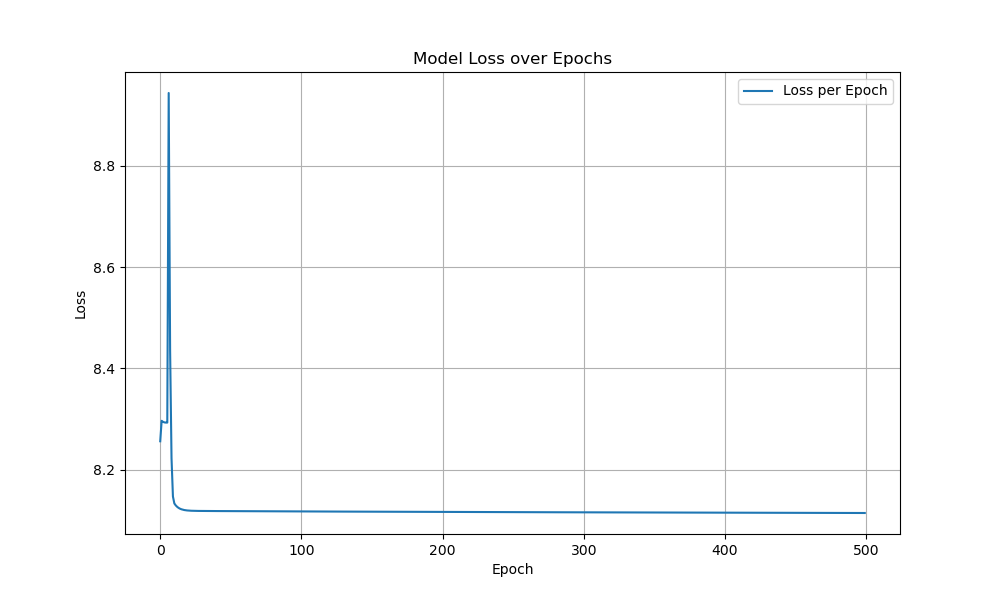
\includegraphics[width=0.8\linewidth]{loss_sgd.png}
    \caption{Loss Function using SGD}
\end{figure}
    
    \item Figure 2 shows the problem of using a higher $\alpha$ value of 0.1. The loss function continuously fluctuated due to overstepping the minimum, and the model did not learn

\begin{figure}[H]
    \centering
    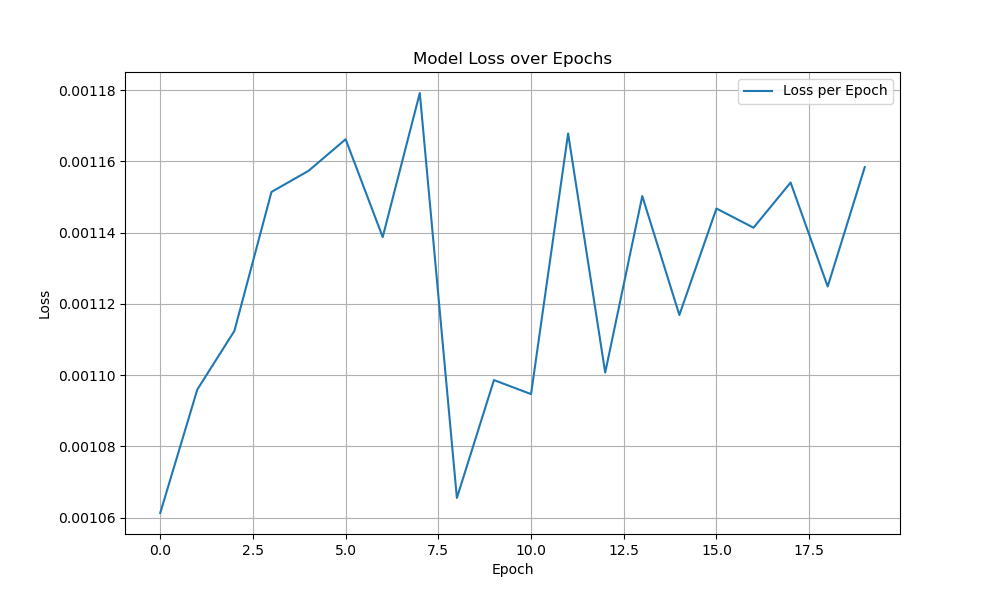
\includegraphics[width=0.8\linewidth]{loss_highalpha.png}
    \caption{Loss Function with alpha=0.1}
\end{figure}
    
    \item Figure 3 shows the final loss function we achieved through training Model 1. The loss decreases and gradually becomes asymptotic, indicating that the model was learning over time. Despite the apparent improvement in accuracy and decreased loss, we noticed the loss value was exceptionally low (even though further testing showed no indication of the model memorizing features). We found this very confusing and eventually realized that this was because our feature values were mostly sparse with many 0s, so the model was learning as much as it could, given the data. We tried training the model on the dataset with 1,219 features and the ones after PCA and variance threshold filtering but did not see a difference in the calculated loss. Overall, as we shall depict in the following section, we tested the model's accuracy using trained and random weights and biases and saw that the model learned adequately, so the abnormally low loss value did not affect Model 1 negatively
\end{itemize}

\begin{figure}[H]
    \centering
    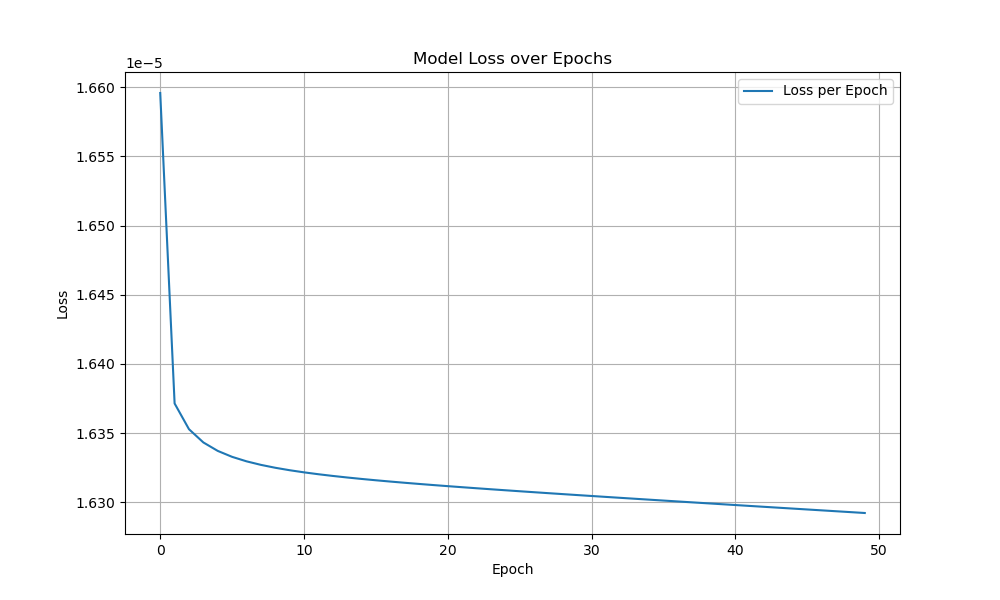
\includegraphics[width=0.8\linewidth]{loss1.png}
    \caption{Final Loss Function}
\end{figure}

\subsubsection{Testing and Evaluation}

After training the model on 50 epochs and ensuring that the loss function had decreased sufficiently, we tested Model 1 on the training and test datasets containing 1,429,898 and 357,475 datapoints respectively. Here are our findings using the \emph{predict\_constrained()} function that applies the validity mask to the predicted probabilities and returns the move class with the maximum probability:

\begin{itemize}
    \item Training Accuracy: 0.7017115906169531
    \item Testing Accuracy: 0.7074145045108049
\end{itemize}

Now, this might not initially seem like a lot and begs the question: what if the model randomly predicts outputs instead of having learned the optimal weights? To counter this argument, we devised an algorithm to generate 100 random weight and bias vectors and calculate the testing accuracy using each parameter pair. We then found the maximum and minimum testing accuracies from the test and compared them to the testing accuracy of the learned parameters:

\begin{itemize}
    \item Maximum Random Testing Accuracy: 0.4941895237429191
    \item Minimum Random Testing Accuracy: 0.4485997622211344
\end{itemize}

Since 0.707 $>$ 0.494, the maximum random testing accuracy over 100 trials, we can affirm with reasonable certainty that Model 1 has indeed learned optimal weights and biases over the training period.

Now, what about whether the model is overfitting or not? Firstly, we have shown that the training and testing accuracy are virtually identical (with the testing accuracy being slightly higher). This finding indicates that the model has not overfitted the training dataset since it performs just as well on the testing dataset. Since the datasets themselves are quite large, we should be able to confirm that the model does not overfit significantly.

However, what if the model has just memorized the bot location features and often predicts the same output since the board configuration was relatively homogenous over the same simulation trial we used to collect data? To answer this question, we tried generating five other test datasets with randomized board start states (in terms of bot, alien, and crew locations) and got similar accuracy values to the training accuracy we found with the original dataset. For example, one of our testing datasets returned an accuracy of 0.7146513365126948, even higher than the testing accuracy on the original dataset. None of our testing datasets returned a lower accuracy than the training accuracy, indicating that the model was not overfitting much and is reasonably generalizable.

\subsubsection{Bot1 vs. Mimic-Bot1}

In this section, we will talk about some specific setups of the Mimic-Bot1 simulation function (along with helper functions) and evaluate the overall performance of Model 1 in practice:

\begin{itemize}
    \item Our Mimic-Bot1 function was almost identical to the Bot1 function defined in Project 2 (and the data collection function defined earlier), but the main difference was the algorithm to predict the next move for the bot given a ship state. Within Bot1, the prediction occurs deterministically, using the logic-based function defined in Project 2 that returns the highest probability neighbor with a 0 alien probability. However, for Mimic-Bot1, the prediction function takes in as parameters the features used in training Model 1 and outputs the model's prediction in the form of a tuple reflecting the best next move
    \item The best-move-finding function initially utilized the \emph{predict\_constrained()} function defined earlier that applies the validity mask to Model 1's predictions based on the input X and returns the highest probability valid neighbor. However, as mentioned earlier, we modified this approach slightly to incorporate a stochastic element in move prediction to avoid endless loops by the bot in some specific scenarios
    \item In the evaluation, we used the same three metrics in Project 2: Average Rescue Moves, Probability of Crew Rescue, and Average Crew Saved. For the hyperparameters, we used the same values as the data collection function: alpha = 0.004, k = 3, timeout = 10,000, with 400 bots for both Bot1 and Mimic-Bot1
    \item Overall, Mimic-Bot1 performed similarly to Bot1 sometimes but was sometimes worse. Here are the results we collected over the span of 20 trials (each containing the average metrics for 20 bots for Bot1 and Mimic-Bot1):
    \begin{itemize}
        \item Bot1: {Average Rescue Moves: [627.05]}, {Probability of Crew Rescue: [0.73]}, {Average Crew Saved: [14.6]}
        \item Mimic-Bot1: Bot1: {Average Rescue Moves: [1768.05]}, {Probability of Crew Rescue: [0.42]}, {Average Crew Saved: [8.4]}
    \end{itemize}
    \item These results suggest that, on average, Bot1 performed significantly better than Mimic-Bot1, but Model 1's predictions weren't completely useless. The large average number of required moves for rescues directly affected the loops that the mimic bot often found itself in, which weren't wholly mitigated despite the addition of stochasticity. Mimic-Bot1 was limited in performance to Bot1's capability since Model1 was trained on simulations using Bot1 itself. Overall, Mimic-Bot1 displayed the ability to traverse the ship effectively and rescue crew members while avoiding aliens, albeit not as well as its deterministic counterpart
\end{itemize}
\section{Model 2}

Similar to the last section, this section goes over the training and testing of Model 2, which is used to predict the bot's performance by determining the probability that the bot will successfully rescue the human. The initial subsection details the general pipeline of Model 2, while the subsequent subsections explain the training and testing processes, respectively. Lastly, the model's efficacy will be discussed through the relevant results.

\subsection{Model 2 Pipeline}

The major components of the Model 2 pipeline are described below:

\begin{enumerate}
    \item Import relevant packages and run the \emph{Bot1.ipynb} notebook to gain access to all the setup functions used for Bot 1 in Project 2. 
    This allowed to set up our simulations. More specifically, we got access to the 30x30 grid, randomly placed the bot, alien, and crew member, and initialized the alien and crew probabilities appropriately. 
    Using these elements, the bot would be able to deterministically determine the next move for the bot, which we would use for data.  
    Like Model 1, it is important to note that we fixed the ship's layout in terms of the default blocked and open cells, meaning only the bot, alien, and crew positions changed throughout simulations. 
    \item Simulate Bot 1 similarly to how it was done in Project 2, but collect relevant feature and output vectors to save in a Pandas dataframe (and eventually store as \emph{model2\_data\_raw.csv}) to be used in training Model 2. 
    \begin{enumerate}
        \item To collect data for this model, we ran 3000 bots where each run ended until the bot saved the crew member or got captured by the alien. More specifically, this was broken into 30 iterations per simulation and 100 simulations. 
         \item From this, we collected a total of 2,952,477 data points. 
         \item For all simulations, the values for the parameters were alpha = 0.004 and k = 3.
         \item The average results from the data collection for Model 2 were similar to the metric results for the simulations for Model 1. 
    \end{enumerate}
    \item Preprocess the data and create training data and testing data splits using the input matrix X and output vector y. Note that the validity mask was unnecessary here as the output space differed. The following steps were taken:
        \begin{enumerate}
        \item Read data from the model2\_data\_raw.csv file and ensure that the shape and structure of the data is as expected. 
        \item Remove duplicate rows/entries from the input matrix X to handle redundancy. Like with Model 1, this step helps to make sure that the model does not become biased by overfitting to the entries that are occurring the most in the data. After this step, the number of data points was reduced to 700,019. 
        \item Modify the feature vectors to ensure that it captures the input information as intended. For this model, no such changes were implemented as we were confident in the current state of the feature vectors.
        \item Partition the data into the input matrix \textit{model2df} and an output vector. From the original data matrix, the output is the last column, and the rest of the columns are the input matrix. In other words, the output vector corresponds to the binary label of whether the bot was successful in rescuing the crew, and the input matrix consists of the other features collected. 
        \item Create training and test matrices by doing an 80/20 split of the \textit{model2df} matrix. For this model, it is important to note that data imbalance was a legitimate concern, given that there was potential for the input data to have a large number of data points that were successes (bot rescued the crew member). To remedy this, we attempted different approaches that I will explain further in the input space section. 
        \end{enumerate}
        \item Train the logistic regression model using the input matrix and input vector (X.train + y.train). Each time, keep track of the updated W and b values. The hyperparameters used in the final training of Model 2 are as follows: 
        \begin{enumerate}
            \item alpha (learning rate) = 0.005
            \begin{itemize}
                \item We tried 0.01 and 0.001, but 0.005 seemed to be the best. In our observations, 0.005 ensured the model did not get stuck at a local minimum quickly and that the model was learning, which was observed by looking at the loss. 
            \end{itemize}
            \item epochs = 50
            \begin{itemize}
                \item 50 proved to be an ideal number for the number of epochs so that the loss decreased incrementally till it became asymptotic. 
            \end{itemize}
        \end{enumerate}
        \item Test Model 2 on the testing data set with the updated W and b values and calculate the accuracy of correctly predicting whether the bot successfully rescues the crew. 
        \begin{itemize}
        \item Similar to model 1, we confirmed that the model was truly learning by using randomized weights and biases and averaging the results over 100 calculations. There was a significant improvement in training and testing accuracy using the trained weights over the random weights.  
        \end{itemize}
    
\end{enumerate}

\subsection{Training Process}
This section covers the training process for Model 2, including the input and output features, the model space, the loss function, and the training algorithm we used.

\subsubsection{Input Space}
The input features used for our data can be described as follows: 
\begin{enumerate}
\item Similar to Model 1, the bot's current x and y coordinates are represented as two individual integer features \textit{bot\_x} and \textit{bot\_y}. 
\item The alien probabilities, or the probability of an alien being present, for all surrounding cells and the current cell that the bot is in. Particularly, they are denoted as \textit{alien\_up}, \textit{alien\_down}, \textit{alien\_left}, \textit{alien\_right}, and \textit{alien\_stay}. Similar to Model 1, we attempted to use a different feature representation of this information. 
\begin{itemize}
    \item The approach of using the complete alien probability matrix after flattening it slowed down our data collection phase. As mentioned, this resulted in around 1200 features. However, most importantly, we did not see a significant increase in the accuracy of the model, even after filtering data according to variance and utilizing PCA in attempt to reduce the dimensionality to a reasonable size. This led us to abandon this approach. 
\end{itemize}
\item Similar to the alien probabilities, the crew member probabilities for the bot's cell and surrounding cells were used as input features. They were labelled as \textit{crew\_up}, \textit{crew\_down}, \textit{crew\_left}, \textit{crew\_right}, and \textit{crew\_stay}. 
\begin{itemize}
    \item It is important to note that \textit{crew\_stay} was kept as a feature as it was helpful in streamlining the data collection process. Most importantly, we confirmed by checking that removing it did not affect the accuracy of the model almost at all. 
    \item Similar to Model 1, normalizing the crew probabilities allowed this feature to be more impactful because without doing this, the crew probabilities often had non-zero values.  
\end{itemize}
\item Two features represented the result of running the alien and crew detectors. Labeled as \textit{alien\_detected} and \textit{crew\_detected}, these features consisted of binary values indicating whether a crew beep or alien beep was heard, respectively. 
\begin{itemize}
    \item Similar to Model 1, removing these features saw a decrease in accuracy due to the possible reason of the data being too sparse. Including these features helped with the handling the existing variance in the data. 
\end{itemize}

\item Overall, our final Model 2 was trained on 14 distinct features stored as integers and float32 values, as depicted above. 
\end{enumerate}
\subsubsection{Data Imbalance}
Upon initial inspection of the input data we collected, it was evident that there was an imbalance in the number of data points for each of the two classes. As mentioned, one class represents that the bot was successful in rescuing the crew, and the other class represents the bot failing in this regard. There seemed to be many more data points that corresponded to the bot being successful, almost twice as many points than the other class. To remedy this, we tried two different approaches. 
\begin{enumerate}
    \item The first approach was to account for this imbalance directly when creating the training and test splits. Since the class 0 or unsuccessful was the class with the smaller number of points, we created a training matrix by concatenating all data points in the original matrix that had an output value of 0 with 50\% of the data points that had 1 as the output value. Given the breakdown of the data points by class in the original matrix, this approach yielded a final training matrix that was around 80\% in size of the original data matrix. We then randomly sampled 20\% of the original data matrix to create the test matrix and complete the 80/20 split. However, this approach saw a significant decrease in accuracy compared to when using the other approach. Specifically, we saw about a 33\% decrease in accuracy in comparison. Initially, we thought this could be because the size of the training set was not big enough to learn the weights meaningfully. However, even after collecting more data, we observed a similar reduced accuracy. As a result, we chose to abandon this approach. 
    \item The approach we ended up utilizing was assigning weights to each class. The weights would essentially account for the varied distribution of data between the classes when the model is learning from the training data. A higher weight for the smaller class, which was the unsuccessful class in this case, would allow the model to learn to classify the class better by penalizing wrong classifications proportionately. We calculated the weights using the following formula: 
    \begin{itemize}
        \item $w_j = \frac{\emph{number of samples for total}}{\emph{number of samples for classes} * \emph{number of samples for class j}} $
    \end{itemize}
    Specifically, we used a weight of 1.556 for class unsuccessful and 0.737 for class successful. After this modification, we confirmed that the model was learning through analysis of the loss and accuracy.  
\end{enumerate}
\subsubsection{Output Space}
The output space for Model 2 consisted of a binary value that indicated whether the state of the bot that was represented through the 14 input features was part of a successful bot run or not. In other words, a 1 meant that this state of the bot was part of a run where the bot rescued the crew, while a 0 meant that this state was part of a run where the bot got captured. 
\begin{itemize}
    \item It is important to note that this approach streamlined the process of collecting input data as each iteration of the bot during a single run could be used as a data point. By doing this, we did not have to run as many simulations of the bot. 
    \item At the same time, this also introduced the effect of redundant data points as the bot often was at a same state between different simulations. As mentioned, this was handled by removing duplicates from the input data. 
\end{itemize}
\subsubsection{Model Space}
To map from the input to the output, we considered a binary logistic regression with sigmoid activation. The steps we followed for the logistic regression model is as follows: 
\begin{enumerate}
    \item During training, the model receives an input vector $X_i$, and uses a linear combination of the vector with weights (W) and bias (b) to compute the output $z = X_i \cdot W + b$. 
    \item The output is then transformed into probabilities for each class via the sigmoid function. It is important to note that there are two classes implicitly, although explicitly only one class is indicated since the probability for the other class can be computed from it. 
    \begin{itemize}
        \item sigmoid($z_j$) = $\frac{1}{1 + e^{-z_j}}$
    \end{itemize}
    This ensures that the probability is distributed over the 2 classes. 
    \item Bonus:
    \begin{itemize}
        \item For our bonus, we used the scikit-learn \emph{LogisticRegression} library to create a binary model using a \emph{lbfgs} (Limited-memory Broyden-Fletcher-Goldfarb-Shanno) solver due to the extensive training dataset. The scikit-learn model also uses the sigmoid activation function I mentioned earlier and uses L2 regularization. We used the same dataset as the logistic regression model we built from scratch. All the other processes were identical.
    \end{itemize}
\end{enumerate}
\subsubsection{Loss}
As a binary classification model, Model 2 uses a cross-entropy loss function that measures the difference between the true and predicted probability distributions for the classes as follows: 
\begin{enumerate}
    \item As parameters, we input the predicted classification of whether the bot was successful or not and the true classification of successful and unsuccessful. 
    \item As mentioned, a validity mask was not necessary here like it was for Model 1. It is important to note that the predicted probability vector $\hat{y}$ is already normalized for the probability distributions for each data point. 
    \item After that, the cross entropy loss is calculated for each data point using the true output vector \emph{y}, predicted output vector  $\hat{y}$, and class weights. 
    \begin{itemize}
        \item $L(y, \hat{y}) = - \Sigma_{i=1}^{2} w \cdot y_i \cdot log(\hat{y_i} + \epsilon)$
        \item In this case, $\epsilon$ refers to a small constant (1e-15) to ensure that log(0) is not being calculated, and $L(y,\hat{y})$ is the loss for that particular datapoint. 
        \item It is important to mention again that the two classes were explicitly represented rather than one class where the other class can be explicitly calculated. Hence, the summation to i = 2. 
        \item Additionally, we modified the output vector into a hot encoding representation to represent two classes. For example, if the output vector was 1, the modified representation was 0 1. 
    \end{itemize}
    \item Lastly, the sum of the losses for each data point is averaged by dividing by the number of data points (n). 
    \item Bonus:
    \begin{itemize}
        \item Like with Bonus for Model 1, we did not define the loss function explicitly since we used the default scikit-learn \emph{LogisticRegression} library. Since we used L2 regularization, the understanding is that a penalty is added to the loss function equal to the sum of the squared values of the calculated weights with a specific regularization strength.
    \end{itemize}
\end{enumerate}
\subsubsection{Training Function}
Like Model 1, the training function uses gradient descent to minimize the cross-entropy loss function. The algorithm iteratively updates the class weights and biases to yield the lowest possible loss value by doing the following: 
\begin{enumerate}
    \item As parameters, we plugged in the true vector y, predicted output vector $\hat{y}$, and the input matrix X. Note the weights were included internally in the function. 
    \item We calculated the gradient of the loss function with respect to the weights W and bias b as follows:
    \begin{itemize}
        \item $\nabla_{W} L = \frac{1}{n} X^{T} \cdot ((\hat{y} - y) \cdot w)$
        \item $\nabla_{b} L = \frac{1}{n} \Sigma_{i=1}^{n} ((\hat{y_i} - y_i) \cdot w)$
    \end{itemize}
    Here, $X$ is the input matrix of size $n \times m$, and $\hat{y}$ and $y$ are the predicted and true output vectors of size $n \times 2$ (since there are 2 classes in the one-hot-encoding). $L$ is the loss function that was calculated before
    \item The gradient of the loss function with respect to $W$ and and $b$ is then used to update the weights and bias in the following way:
    \begin{itemize}
        \item $W = W - \alpha \cdot \nabla_{W} L$
        \item $b = b - \alpha \cdot \nabla_{b} L$
    \end{itemize}
    As mentioned, $\alpha$ (0.005) is the training algorithm's learning rate. We found that higher learning rates caused the loss to oscillate, while smaller learning rates rendered the model to be significantly slow in learning.  The former could have because the model was possibly overstepping. 
    \item This algorithm was used in each iteration or epoch to train the model on the entire dataset. Like Model 1, we tried out stochastic gradient descent here as well. However, we observed that the loss function decreased more steadily by utilizing full-batch gradient descent. Overall, we finally trained Model 1 for 50 epochs, which allowed the loss to decrease and eventually become asymptotic. 
    \item Bonus:
    \begin{itemize}
        \item Once again, we did not explicitly define the training function since we used the default scikit-learn \emph{LogisticRegression} library. We utilized \emph{lbfgs}, or Limited-memory Broyden-Fletcher-Goldfarb-Shanno, which uses a similar process but is much more memory-efficient as it is geared for extensive data sets. 
    \end{itemize}
\end{enumerate}
\subsection{Testing Process and Results}
This section is an analysis of the testing process we used and the simulation results we got. 
\subsubsection{Results}
These were some of the plots that were generated when analyzing the loss function while the model was being trained. 
\begin{itemize}
\item Figure 1 shows the change in the loss function when the $\alpha$ value was relatively high. Specifically, the $\alpha$ values were 0.01 and 0.05. Both values resulted in a plot like this. After the first 10 epochs, the loss oscillates between values around 5 and values around 0. As mentioned, this could be due to the model overstepping and missing the local maxima.  
        \begin{figure}[H]
        \centering
        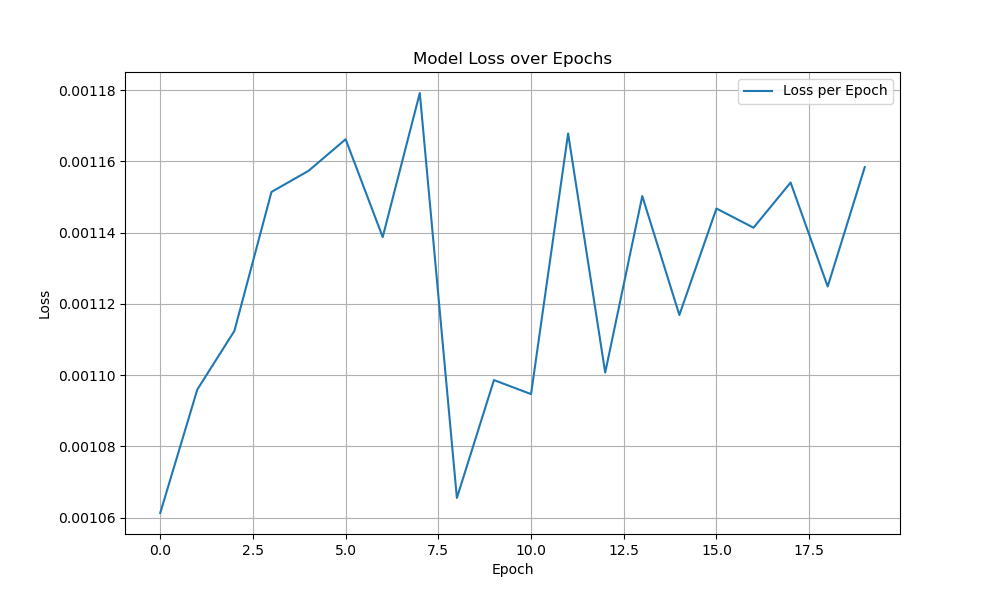
\includegraphics[width=0.8\linewidth]{loss_m2highalpha.png}
        \caption{Loss Function using $\alpha = 0.01$}
        \end{figure}
       
    \item Figure 2 shows the final loss function we achieved through training Model 2. As mentioned, the number of epochs was 50, and $\alpha$ was 0.005. The loss decreased at a relatively greater rate in the early epochs before decreasing gradually after around 15 epochs. Eventually, the loss became asymptotic. Evidently, this suggests that the model was learning. We confirmed this suggestion by testing the accuracy of the model. 
         \begin{figure}[H]
        \centering
        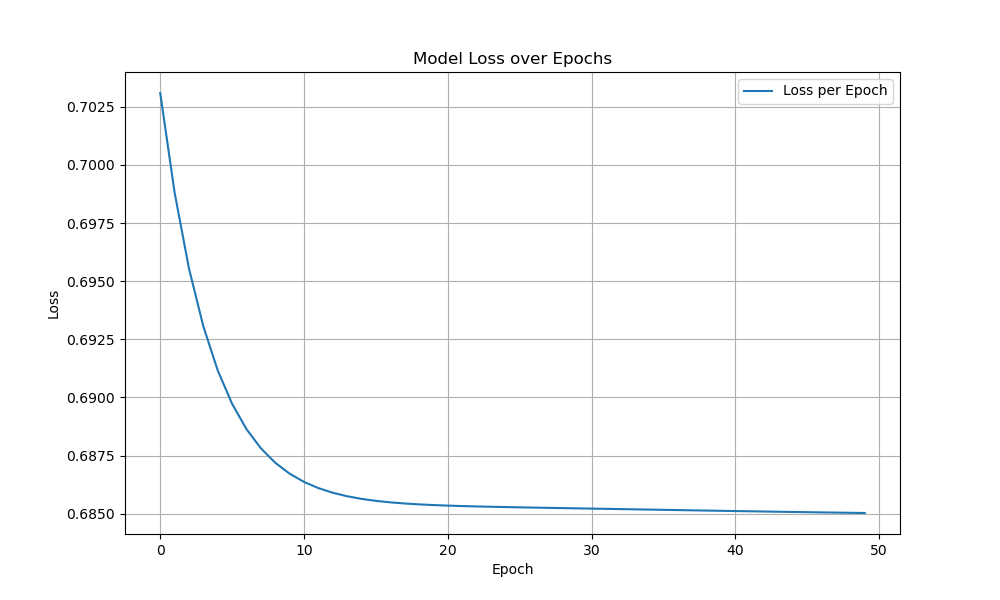
\includegraphics[width=0.8\linewidth]{loss_m2final.png}
        \caption{Final Loss Function}
        \end{figure}
\end{itemize}
\subsubsection{Testing and Evaluation}
After training the model on 50 epochs and observing the decrease in the loss to an asymptotic level, we tested Model 2 on the training and test datasets containing 560,015 and 140,003 data points, respectively. It is important to note that in this process, the predicted result of either successful or unsuccessful was determined as the class with the maximum probability:
\begin{itemize}
    \item Training Accuracy: 0.6786282510289903
    \item Testing Accuracy: 0.6805640221995243
\end{itemize}

To ensure that the model had learned and was not randomly predicting output, we compared the model to the testing accuracy determined using random weights and bias vectors, similar to how Model 1 was checked. Specifically, we looked at the maximum and minimum testing accuracy over 100 randomly generated weights and biases.  
\begin{itemize}
    \item Maximum Testing Accuracy: 0.5007205164147389
    \item Minimum Testing Accuracy: 0.3210324064484332
\end{itemize}
Since the model's testing accuracy is significantly higher in comparison, it can be evaluated that the model has learned optimal weights and bias. 

The result of the testing accuracy of the model being close to the training accuracy shows that the model is not overfitting. To confirm that the bot is not memorizing features and just providing the same output, we ran this model for other test data sets that corresponded with different board start states, like with Model 1. We checked with around 5 different test data sets. For 3 out of the 5 test data sets, the testing accuracy was around the same as the testing accuracy recorded for the original test data set. This leads to the conclusion that the bot is not overfitting and is reasonably capable of learning optimal weights and bias. 

\section{Model 3}

This section is dedicated to our training, testing, and incremental improvement of Model 3, which involves using reinforcement learning with an ACTOR-CRITIC framework to enable the ACTOR to predict the best next move for the bot based on the current grid configuration and the CRITIC's prediction of the move's success rate. The subsections shall include the following essential information: the general pipeline of Model 3, the specifications of ACTOR and the CRITIC networks, a thorough analysis of learning and improvement, and a presentation of the testing process along with any relevant results.

\subsection{Model 3 Pipeline}

Because we went into great detail on Model 1 and Model 2, Model 3, which can be considered a combination of the two, is not unique in its data collection, preprocessing, and pretraining. Therefore, I have outlined the general pipeline of Model 3 below, along with any specific steps taken:

\begin{enumerate}
    \item Import relevant packages and ensure that the dataset used to train Model 1 (\emph{model\_data\_raw.csv}) has been appropriately configured and loaded for Model 3 as a Pandas dataframe called \emph{pretrain\_data}
    \item Preprocess the collected pre-training data, similar to Model 1, and perform train/test splits for the input matrix X and output vector y. We also generated a validity mask for the output vector at this pipeline step, but more later. The following general preprocessing steps were taken:
    \begin{enumerate}
        \item Read the data from \emph{model\_data\_raw.csv} and ensure that the shape is consistent and the data is loading correctly
        \item Remove duplicates from the data to streamline the dataset and remove redundancy. Without this step, the model might memorize frequently occurring data points or become skewed/biased. After this step, the total data points are reduced to 1,787,373
        \item Separate the data into the input matrix X and the output vector y (with the output being the last column and the input being all the other columns). Since we decided to use a PyTorch neural network for ACTOR, we had to slightly modify the output vector to convert the one-hot-encoded lists to integers based on the class indices (similar to the approach in Model 1 Bonus)
        \item Divide the X and y dataframes into train and test sets with an 80/20 split, respectively, using the scikit-learn \emph{train\_test\_split()} function. At this point, we also checked that all five classes were equally represented in each set
        \item Then, generate the validity mask vector dataframes for the train and test sets. Each row in the validity mask corresponds to the same row in the X\_pt\_train and X\_pt\_test datasets and represents the neighbors the bot can move to, given the board's open and closed cells. The following process was used to generate this validity mask:
        \begin{enumerate}
            \item For any given datapoint, use the bot\_x and bot\_y features (that represent the bot's current coordinates) along with an empty grid state to determine what neighbor cells count as valid moves for the bot
            \item Each datapoint in the valid dataframes is represented as a boolean list in the form of [$c_1, c_2, c_3, c_4, c_5$] depicting the up, down, left, right, and bot cells, respectively. Each $c_i$ is False if the corresponding relative neighbor is an invalid move and True if the bot can move to it
        \end{enumerate}
        \item Finally, convert the X\_pt\_train and X\_pt\_test datasets into float32 tensor matrices and the y\_pt\_train and y\_pt\_test datasets into long tensors to be used in pre-training the ACTOR network
    \end{enumerate}
    \item Initialize and pre-train the ACTOR network on the X\_pt\_train + y\_pt\_train tensors to allow it to learn the optimal weights to predict the best moves. We used a learning rate of 0.001. I will go into the input, output, and model spaces, as well as the learning techniques, in the next section
    \item Import and run the \emph{Bot1.ipynb} notebook to gain access to all the setup functions used for Bot 1 in Project 2 similar to Model 1 and 2. Collect relevant feature and output vectors to save in a Pandas dataframe (and eventually store as \emph{actor\_data.csv} similar to Model 2 to be used in training the CRITIC network. I shall go into more detail about the exact feature and output vectors in the next section.
    \begin{enumerate}
        \item To collect enough data, we ran 200 bots (i.e., until the bot saved the crew or got captured): 20 iterations per simulation and 10 simulations
        \item Through these simulations, we collected a total of over 840,000 data points
        \item The following hyperparameters were used: alpha = 0.004, k = 3
        \item Note that these values only reflect the initial simulation for our data collection phase. The \emph{actor\_data.csv} file was constantly updated with new data during our reinforcement learning loops
        \item Importantly, and as we shall detail in the next section, the data collection loop now stored the best next move as a feature (unlike in Model 1) and instead had the success rate per move as the output vector
    \end{enumerate}
    \item Initialize and train the CRITIC network on the \emph{actor\_data.csv} collected using the ACTOR network. I shall discuss the CRITIC framework in more detail shortly, so let me first go into more detail about the ACTOR-CRITIC loop that shall serve as the reinforcement learning phase. The CRITIC and ACTOR training loops are run sequentially within an outer loop, and the following processes take place in each loop:
    \begin{enumerate}
        \item The CRITIC loop first takes the existing critic network and Adam optimizer as parameters and generates data based on the predicted moves by the current ACTOR network as \emph{actor\_data.csv}. The data collection takes place over the same hyperparameters and iterations as the original \emph{actor\_data.csv} generation, i.e., 200 bots with alpha = 0.004 and k = 3. Then, it preprocesses the data and trains on it to utilize the updated true success and failure metrics output vector to improve its predictive capabilities. This process is very similar to the training process of Model 2
        \item The ACTOR loop first generates data based on the predicted moves by the current ACTOR network as \emph{critic\_data.csv}. While this data collection takes place over the same hyperparameters and iterations as the CRITIC loop, it stores the predicted moves as the output vector, similar to Model 1. The process then uses the CRITIC network iteratively on the generated \emph{critic\_data.csv} dataset and replaces the predicted move with the highest-success-rated move predicted by CRITIC based on the input features. Then, the ACTOR network trains on the updated dataset to improve its best move prediction capabilities. Finally, the ACTOR network is evaluated based on its accuracy and loss decrease
    \end{enumerate}
    \item Finally, simulate the ACTOR network through a new bot called Mimic-Bot3 that utilizes the network's predictions to determine the next move for the bot by utilizing the same features as the trained model. Here is a general outline of the process:
    \begin{enumerate}
        \item Create the Mimic-Bot3 simulation function identical to the Mimic-Bot1 simulation function, predicting the next move at each timestep by using the ACTOR network with a dataframe input containing features extracted from the current ship configuration
        \item Test the Mimic-Bot3 simulation out against the Bot1 simulation function similar to how the testing was performed for Model 1, and store the collected average metrics for each bot
        \item We ran 400 bots for both Bot 1 and Mimic-Bot3: 20 iterations per simulation and 20 simulations
        \item The following hyperparameters were used: alpha = 0.004, k = 3
        \item Importantly, we calculated a validity mask for every X input, and used a prediction function that applied the validity mask to the output to ensure that the bot would remain within bounds
        \item Later, we added a stochastic element to the prediction provided by ACTOR. In essence, we generated a random number between 1 and 5 and returned a random valid move if the number was 1 (i.e., 20\% of the time). This modification accounted for situations where Mimic-Bot3 got stuck in an endless loop. Consider the following scenario: The bot is in a cell from which the highest probability neighbor is "up," but following the highest probability from "up," the bot is taken back to the original cell. By adding slight randomness, Mimic-Bot3 can escape such loops by taking unexpected actions
    \end{enumerate}
\end{enumerate}

\subsection{ACTOR Network}

In this section, I shall outline the specifications for ACTOR, including the neural network architecture, forward and backpropagation techniques, the loss function, parameter updates, and the training, prediction, and testing functions we used.

\subsubsection{Input Space}

The data that was collected and represented as input features for ACTOR's training are almost exactly the same as Model 1:

\begin{enumerate}
    \item The bot's current x and y coordinates as two individual integer features \emph{bot\_x} and \emph{bot\_y}
    \item The alien probabilities for all neighboring cells (and the current bot cell) as float32 features. They are in the order: \emph{alien\_up}, \emph{alien\_down}, \emph{alien\_left}, \emph{alien\_right}, \emph{alien\_stay} representing the probabilities of the alien being in the up, down, left, right, and bot cells respectively
    \item The crew member probabilities for all neighboring cells (and the current bot cell) as float32 features. They are in the order: \emph{crew\_up}, \emph{crew\_down}, \emph{crew\_left}, \emph{crew\_right} representing the probabilities of the crew member being in the up, down, left, and right cells respectively
    \item Per the professor's announcement, we added features reflecting the distance from the bot's neighboring cells to the two cells with the highest alien and crew member probabilities, respectively. Hence, we included ten additional features: \emph{d\_alien\_up}, \emph{d\_alien\_down}, \emph{d\_alien\_left}, \emph{d\_alien\_right}, \emph{d\_alien\_stay}, \emph{d\_crew\_up}, \emph{d\_crew\_down}, \emph{d\_crew\_left}, \emph{d\_crew\_right}, \emph{d\_crew\_stay} stored as float32 values. We heeded Aravind's announcement on Zulip and made sure that the actual locations for the crew member and alien were not used at any point during this distance calculation process since the maximum probability cell within the crew and alien matrices might not reflect the true locations
    \item The binary values for whether the bot received a beep or not from the alien sensor and crew sensor as two features: \emph{alien\_detected} and \emph{crew\_detected}
\end{enumerate}

Overall, ACTOR was continuously trained on 23 distinct features stored as integers and float32 values, as depicted above

\subsubsection{Output Space}

The output space for ACTOR consisted of the best move made by the bot with a given ship configuration, similar to Model 1 Bonus. The moves are encoded as integers as follows: up = 0, down = 1, left = 2, right = 3, stay = 4

\subsubsection{Model Space}

The ACTOR model architecture is defined below:

\begin{itemize}
    \item The ACTOR model is a PyTorch neural network with three fully-connected layers (one input, one hidden, one output):
    \begin{enumerate}
        \item The first layer transforms the input features to a 128-neuron hidden layer using a linear transformation as the weighted sum of the inputs plus the bias vector. Additionally, the ReLU activation function introduces non-linearity to ACTOR, allowing it to learn complex patterns from the data. Essentially, ReLU outputs the input directly if positive and 0 if negative (i.e., $f(x) = \max(0, x)$)
        \item The second layer reduces the dimension to five, corresponding to each of the output labels depicting possible actions
        \item The third layer applies the Softmax function to the output layer to convert logits to probabilities and provide a distribution over the possible actions. Essentially, given a logit vector $z$ with five elements, the Softmax function computes:
        \begin{itemize}
            \item Softmax($z_i$) = $\frac{e^{z_i}}{\Sigma_{k=1}^5 e^{z_k}}$
        \end{itemize}
        This computation is done for each element $z_i$ of the logit vector
    \end{enumerate}
\end{itemize}

\subsubsection{Loss}

Similar to Model 1, ACTOR uses a cross-entropy loss function that measures the difference between the true and predicted probability distributions for the classes in the following way:

\begin{itemize}
    \item Given the predicted probability distribution $\hat{y}$ from the Softmax output, where each element of $\hat{y}$ is the predicted probability of each class, the cross-entropy loss for a datapoint is calculated as such:
    \begin{itemize}
        \item $L = - log(\hat{y_i})$
        \item $i$ is the index of the true class label for the datapoint
    \end{itemize}
    \item The total loss is then calculated as the average of each of these losses
\end{itemize}

\subsubsection{Training Algorithm}

The training algorithm for ACTOR involves the following steps:

\begin{enumerate}
    \item Forward Propagation:
    \begin{itemize}
        \item The model receives the input vector X (representing the current state) and computes the output through its layers. The output of each layer is calculated as:
        \begin{itemize}
            \item For a layer $l$, the output $O_l$ is given by $O_l = f(W_l \cdot O_{l - 1} + b_l)$
            \item In this case, $W_l$ and $b_l$ are the calculated weights and biases, $O_{l - 1}$ is the output of the previous layer, and $f$ is the activation function (ReLU for the first layer, and Softmax for the third)
        \end{itemize}
    \end{itemize}
    \item Loss Calculation:
    \begin{itemize}
        \item The cross-entropy loss is then calculated using the loss function defined in the previous subsection
    \end{itemize}
    \item Backward Propagation:
    \begin{itemize}
        \item Then we calculate the gradient of the loss function with respect to the weights $W$ and bias $b$ as follows:
        \begin{itemize}
            \item $\nabla_{W} L = \frac{1}{n} X^{T} \cdot (\hat{y} - y)$
            \item $\nabla_{b} L = \frac{1}{n} \Sigma_{i=1}^{n} (\hat{y_i} - y_i)$
        \end{itemize}
        In this case, $X$ is the input matrix of size $n \times m$, and $\hat{y}$ and $y$ are the predicted and true output vectors of size $n \times 1$. Additionally, $L$ is the loss function that was calculated earlier
    \end{itemize}
    \item Parameter Update:
    \begin{itemize}    
        \item Finally, after the gradient of the loss function with respect to both $W$ and $b$ have been calculated, the model uses them to update the weights and bias in the following way:
        \begin{itemize}
            \item $W = W - \alpha \cdot \nabla_{W} L$
            \item $b = b - \alpha \cdot \nabla_{b} L$
        \end{itemize}
        The $\alpha$ used in these updates refers to the learning rate of the training algorithm, which we set to 0.001
    \end{itemize}
\end{enumerate}

\subsection{CRITIC Network}

In this section, I shall outline the specifications for CRITIC, including the neural network architecture, forward and backpropagation techniques, the loss function, parameter updates, and the training, prediction, and testing functions we used.

\subsubsection{Input Space}

The data that was collected and represented as input features for CRITIC's training are almost exactly the same as ACTOR, with one major addition:

\begin{enumerate}
    \item The bot's current x and y coordinates as two individual integer features \emph{bot\_x} and \emph{bot\_y}
    \item The alien probabilities for all neighboring cells (and the current bot cell) as float32 features. They are in the order: \emph{alien\_up}, \emph{alien\_down}, \emph{alien\_left}, \emph{alien\_right}, \emph{alien\_stay} representing the probabilities of the alien being in the up, down, left, right, and bot cells respectively
    \item The crew member probabilities for all neighboring cells (and the current bot cell) as float32 features. They are in the order: \emph{crew\_up}, \emph{crew\_down}, \emph{crew\_left}, \emph{crew\_right} representing the probabilities of the crew member being in the up, down, left, and right cells respectively
    \item Features reflecting the distance from the bot's neighboring cells to the two cells with the highest alien and crew member probabilities, respectively. Hence, we included ten additional features: \emph{d\_alien\_up}, \emph{d\_alien\_down}, \emph{d\_alien\_left}, \emph{d\_alien\_right}, \emph{d\_alien\_stay}, \emph{d\_crew\_up}, \emph{d\_crew\_down}, \emph{d\_crew\_left}, \emph{d\_crew\_right}, \emph{d\_crew\_stay} stored as float32 values. Once again, we heeded Aravind's announcement on Zulip and made sure that the actual locations for the crew member and alien were not used at any point during this distance calculation process since the maximum probability cell within the crew and alien matrices might not reflect the true locations
    \item The binary values for whether the bot received a beep or not from the alien sensor and crew sensor as two features: \emph{alien\_detected} and \emph{crew\_detected}
    \item The final input feature was the predicted best move by the ACTOR model, encoded as an integer reflecting the class label as follows: up = 0, down = 1, left = 2, right = 3, stay = 4
\end{enumerate}

Overall, CRITIC was continuously trained on 24 distinct features stored as integers and float32 values, as depicted above

\subsubsection{Output Space}

The output space for CRITIC consisted of a binary value that indicated whether the state of the bot represented through the 24 input features was part of a successful bot run, similar to Model 2. In other words, a 1 meant that this state of the bot was part of a run where the bot rescued the crew, while a 0 indicated that this state was part of a run where the bot got captured.

\subsubsection{Model Space}

The CRITIC model architecture is defined below:

\begin{itemize}
    \item The CRITIC model is a PyTorch neural network with three fully-connected layers (one input, one hidden, one output):
    \begin{enumerate}
        \item The first layer transforms the input features to a 128-neuron hidden layer using a linear transformation as the weighted sum of the inputs plus the bias vector. The ReLU activation function also introduces non-linearity to CRITIC, allowing it to learn complex patterns from the data. Essentially, ReLU outputs the input directly if positive and 0 if negative (i.e., $f(x) = \max(0, x)$). This layer is structured similarly to ACTOR
        \item The second layer reduces the dimension to one, corresponding to the output label depicting the success rate. Instead of having two output labels like Model 2, we decided that having one neuron with a threshold to indicate whether the probability represented success or failure would be more appropriate
        \item The third layer in the CRITIC model applies the Sigmoid function to the output layer. This function maps logits to a range between 0 and 1, aligning with the CRITIC's role of estimating the value of state-action pairs. The sigmoid function is defined mathematically as:
        \begin{itemize}
            \item Sigmoid($z$) = $\frac{1}{1 + e^{-z}}$
        \end{itemize}
        This formula is applied to the output of the final linear layer. Overall, Sigmoid is suitable for binary outcomes or probability estimation of a single event, fitting the CRITIC's purpose
    \end{enumerate}
\end{itemize}

\subsubsection{Loss}

In contrast to the ACTOR model, the CRITIC uses a binary cross-entropy Loss function that measures the difference between the binary true labels and the predicted probabilities.

\begin{itemize}
    \item Given the predicted probability vector $\hat{y}$ from the Sigmoid output, the binary cross-entropy loss for a datapoint is calculated as such:
    \begin{itemize}
        \item $L = - (y \cdot log(\hat{y}) + (1 - y) \cdot log(1 - \hat{y}))$
    \end{itemize}
    \item The total loss is then calculated as the average of each of these losses
\end{itemize}

\subsubsection{Training Algorithm}

The training algorithm for CRITIC involves the following steps:

\begin{enumerate}
    \item Forward Propagation:
    \begin{itemize}
        \item The model receives the input vector X (representing the current state) and computes the output through its layers. The output of each layer is calculated as:
        \begin{itemize}
            \item For a layer $l$, the output $O_l$ is given by $O_l = f(W_l \cdot O_{l - 1} + b_l)$
            \item In this case, $W_l$ and $b_l$ are the calculated weights and biases, $O_{l - 1}$ is the output of the previous layer, and $f$ is the activation function (ReLU for the first layer, and Sigmoid for the third)
        \end{itemize}
    \end{itemize}
    \item Loss Calculation:
    \begin{itemize}
        \item The binary cross-entropy loss is then calculated using the loss function defined in the previous subsection
    \end{itemize}
    \item Backward Propagation:
    \begin{itemize}
        \item Then we calculate the gradient of the loss function with respect to the weights $W$ and bias $b$ as follows:
        \begin{itemize}
            \item $\nabla_{W} L = \frac{1}{n} X^{T} \cdot (\hat{y} - y)$
            \item $\nabla_{b} L = \frac{1}{n} \Sigma_{i=1}^{n} (\hat{y_i} - y_i)$
        \end{itemize}
        In this case, $X$ is the input matrix of size $n \times m$, and $\hat{y}$ and $y$ are the predicted and true output vectors of size $n \times 1$. Additionally, $L$ is the loss function that was calculated earlier
    \end{itemize}
    \item Parameter Update:
    \begin{itemize}    
        \item Finally, after the gradient of the loss function with respect to both $W$ and $b$ have been calculated, the model uses them to update the weights and bias in the following way:
        \begin{itemize}
            \item $W = W - \alpha \cdot \nabla_{W} L$
            \item $b = b - \alpha \cdot \nabla_{b} L$
        \end{itemize}
        The $\alpha$ used in these updates refers to the learning rate of the training algorithm, which we set to 0.001
    \end{itemize}
\end{enumerate}

\subsection{Reinforcement Learning}

This section will present the findings from the reinforcement learning loop, including evidence that the CRITIC and ACTOR models learned through training.

\subsubsection{CRITIC Loop}

As explained earlier, the CRITIC loop generates data leveraging the ACTOR network's predictive capabilities and then trains the CRITIC network. Throughout our 20 iterations of reinforcement learning, we observed that the CRITIC network was continuously able to learn from the data and update its weights and biases, and we verified this improvement via loss-decrease plots. For the sake of space, we shall not include each plot, but here are two of them taken during the first and final iterations:

\begin{figure}[H]
    \centering
    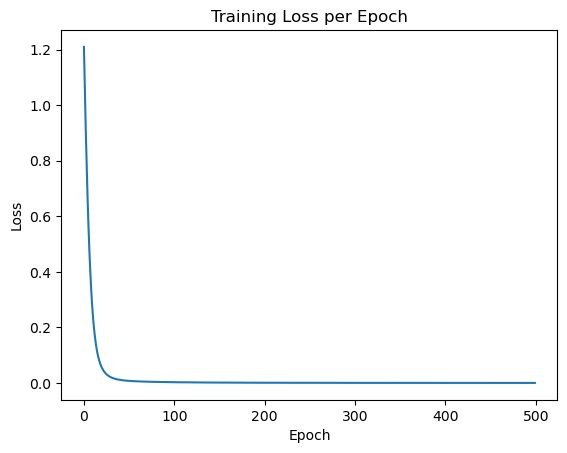
\includegraphics[width=0.4\linewidth]{criticloss.png}
    \caption{CRITIC Loss Decrease (i=1)}
\end{figure}

\begin{figure}[H]
    \centering
    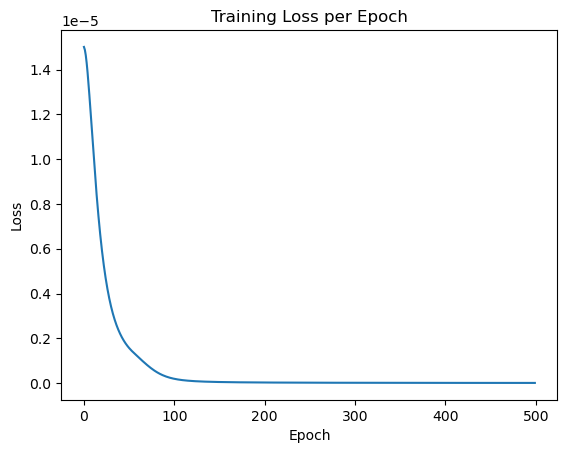
\includegraphics[width=0.4\linewidth]{criticloss2.png}
    \caption{CRITIC Loss Decrease (i=20)}
\end{figure}

\subsubsection{ACTOR Loop}

Similarly, the ACTOR loop generates data leveraging the ACTOR network's predictive capabilities and then uses the CRITIC network's predictions to optimize the dataset, which it subsequently trains on. Throughout our 20 iterations of reinforcement learning, we observed that the ACTOR network was also continuously able to learn from the data and update its weights and biases, and we verified this improvement via loss-decrease plots. For the sake of space, we shall not include each plot, but here are two of them taken during the first and final iterations:

\begin{figure}[H]
    \centering
    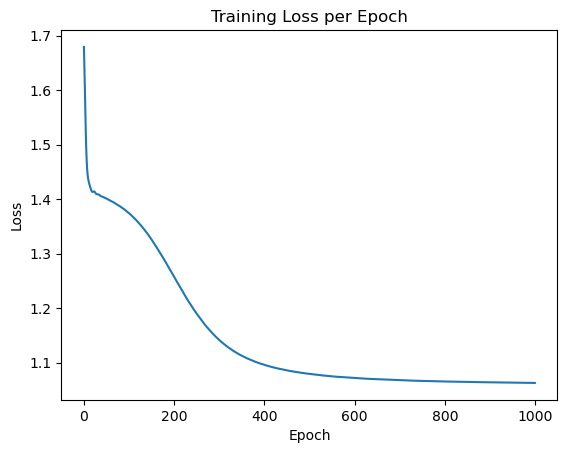
\includegraphics[width=0.4\linewidth]{actorloss.png}
    \caption{ACTOR Loss Decrease (i=1)}
\end{figure}

\begin{figure}[H]
    \centering
    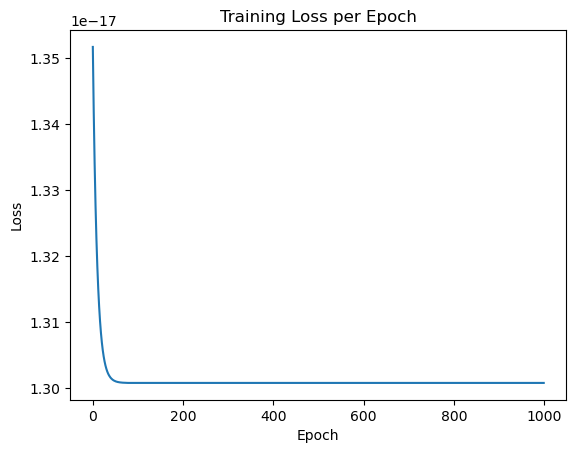
\includegraphics[width=0.4\linewidth]{actorloss2.png}
    \caption{ACTOR Loss Decrease (i=20)}
\end{figure}

\subsubsection{ACTOR Improvement}

After every reinforcement learning iteration, we compared the metrics collected from simulating the ACTOR network during data collection and generated plots to verify ACTOR improvement:

\begin{figure}[H]
    \centering
    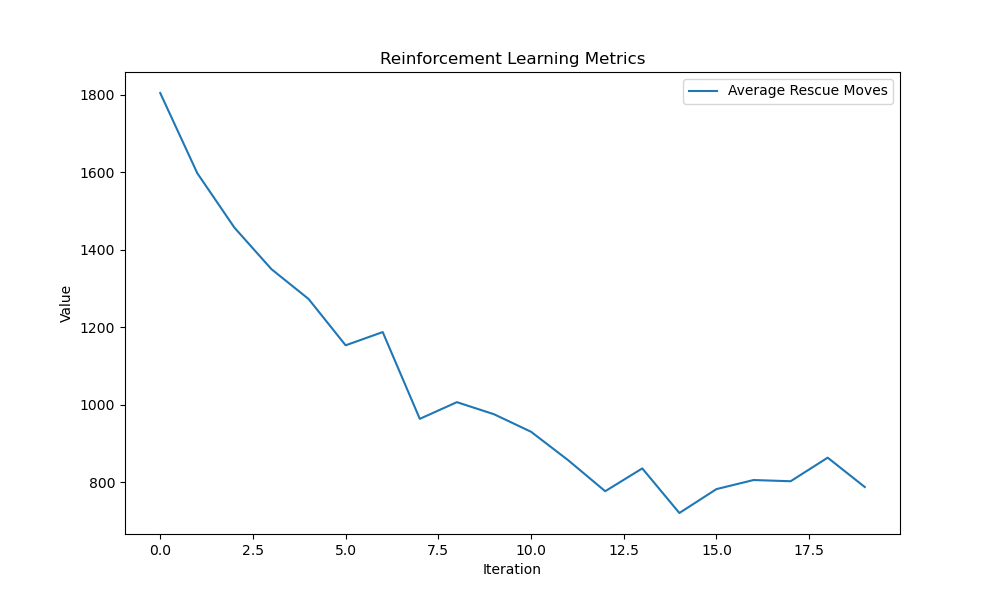
\includegraphics[width=0.8\linewidth]{actormoves.png}
    \caption{ACTOR Average Rescue Moves}
\end{figure}

This figure clearly shows the ACTOR's performance increasing in terms of the number of moves needed to rescue the crew member over the 20 training sessions

\begin{figure}[H]
    \centering
    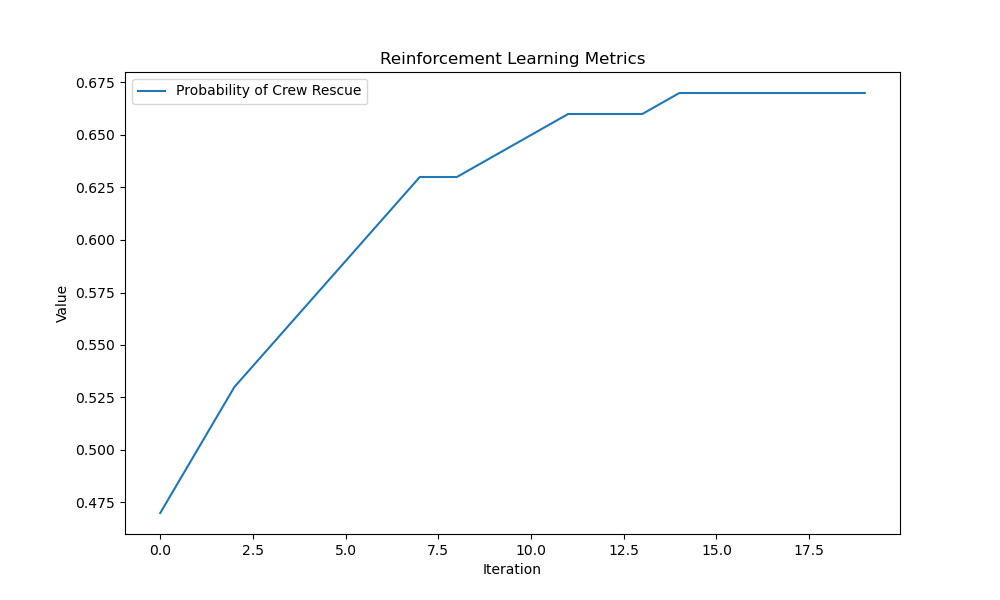
\includegraphics[width=0.8\linewidth]{actorprob.png}
    \caption{ACTOR Probability of Crew Rescue}
\end{figure}

Similarly, this figure clearly shows that the ACTOR gradually had a higher probability of crew rescue over the 20 training sessions

\begin{figure}[H]
    \centering
    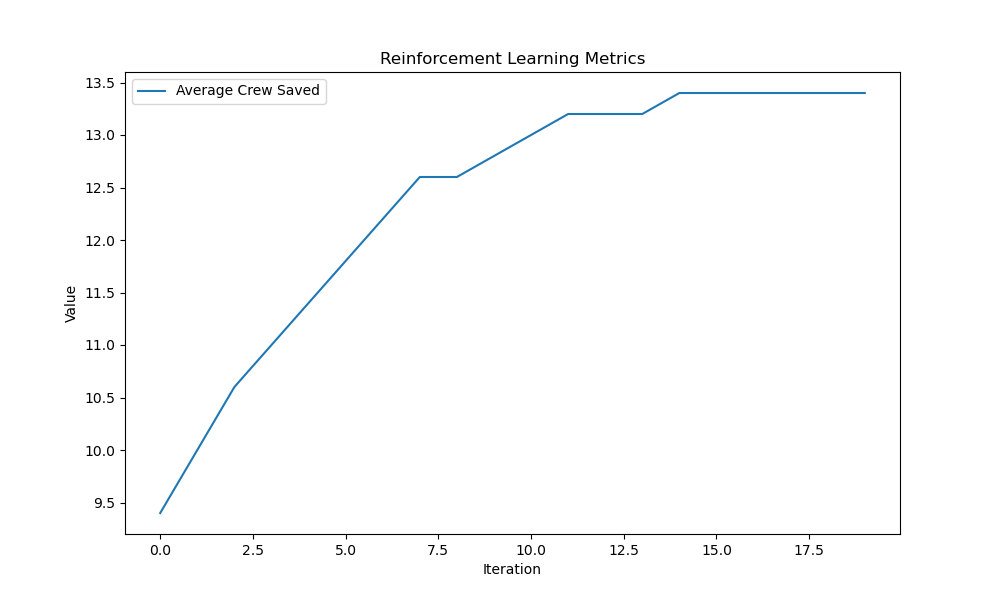
\includegraphics[width=0.8\linewidth]{actorcount.png}
    \caption{ACTOR Average Crew Saved}
\end{figure}

Finally, we can also see that the ACTOR gradually saves more crew members per simulation due to reinforcement learning

\subsection{Testing Process and Results}

This section will highlight our simulation results and an overall analysis of our findings.

\subsubsection{Bot1 vs. Mimic-Bot3}

In this section, we will talk about some specific setups of the Mimic-Bot3 simulation function and evaluate the overall performance of ACTOR in practice:

\begin{itemize}
    \item Our Mimic-Bot3 function was almost identical to the Mimic-Bot1 function defined for Model 1, and the only difference was the algorithm to predict the next move for the bot given a ship state. Similar to the pre-training data generation simulation, we used a prediction function for the PyTorch neural network (with an applied validity mask) that returned the best next move
    \item As mentioned earlier, we also modified this approach slightly to incorporate a stochastic element in move prediction to avoid endless loops by the bot in some specific scenarios
    \item In the evaluation, we used the same three metrics in Model 1: Average Rescue Moves, Probability of Crew Rescue, and Average Crew Saved. For the hyperparameters, we used the same values as the data collection function: alpha = 0.004, k = 3, timeout = 10,000, with 400 bots for both Bot1 and Mimic-Bot3
    \item Overall, Mimic-Bot3 performed similarly to Bot1. Here are the results we collected over the span of 20 trials (each containing the average metrics for 20 bots for Bot1 and Mimic-Bot3):
    \begin{itemize}
        \item Bot1: {Average Rescue Moves: [733.34]}, {Probability of Crew Rescue: [0.69]}, {Average Crew Saved: [13.8]}
        \item Mimic-Bot3: {Average Rescue Moves: [835.26]}, {Probability of Crew Rescue: [0.66]}, {Average Crew Saved: [13.2]}
    \end{itemize}
    \item These results suggest that, on average, although Mimic-Bot3 significantly outperformed Mimic-Bot1, it unfortunately did not perform better than Bot1. However, given more time, we are confident that it would be possible to find the optimal features, hyperparameters, and model architectures to defeat Bot1 once and for all!
\end{itemize}

\end{document}